%!TEX root = practicum4.tex
\subsection{Creating the DCEL}
To create a DCEL one needs a couple of base classes, namely \t{Vertex}, \t{HalfEdge} and \t{Face}. 

\subsubsection*{Vertex}
	The definition of the class \t{Vertex} and its methods that are pertinent now are presented in \autoref{lst:a:vertex}. In line with the provided definition a \t{Vertex} has a set of coordinates representing its location, \t{coordinates}, and an edge, \t{incident_edge}, that has the \t{Vertex} as its origin.

	I have overridden the equality definition since using the default definition could lead to infinite recursion. As the default compares all attributes of the class, which would mean comparing two \t{Vertex}'s and two \t{HalfEdge}s. Comparing two \t{HalfEdge}s means comparing, among others, its \t{origin}s which would lead to comparing two \t{Vertex}s which would lead to comparing two \t{HalfEdge}s and so on and so forth.

	Since each \t{Vertex} is uniquely defined by its \t{coordinates} we only compare those when checking the equality of two \t{Vertex}s.
	\lstinputlisting[firstline=14, lastline=28, label={lst:a:vertex}, caption={The definition of the class \t{Vertex}.}]{../vertex.py}

\subsubsection*{HalfEdge}
	A \t{HalfEdge} is a directed edge which is represented by its \t{origin}, a \t{Vertex} and a \t{twin}, which is the \t{HalfEdge} with this \t{HalfEdge}'s origin as its destination and this \t{HalfEdge}'s destination as its origin. The implementation of the class \t{HalfEdge} and the methods relevant to this discussion are presented in \autoref{lst:a:halfEdge}.

	Furthermore each \t{HalfEdge} stores an incident face and a next and previous edge. The \t{incident_face} is the face that is to the left-handed side when walking along this edge. The attributes \t{nxt} represent the edge one should take on arriving on the \t{HalfEdge}'s destination when traversing the boundaries of its \t{incident_face}, \t{prev} is the \t{HalfEdge} one came from on the same walk. 

	The method \t{get_destination} returns the destination of the \t{HalfEdge} this is the same as the \t{origin} of its \t{twin}.

	The \t{__eq__} method of \t{HalfEdge} has been overridden to avoid infinite recursion when comparing \t{HalfEdge}'s and to make it possible to compare an \t{HalfEdge} without the \t{nxt}, \t{incident_face} or \t{prev} property. This will not lead to any problems since an \t{HalfEdge} is uniquely defined by its origin and destination.

	\todo[inline]{Edges zijn niet uniquely defined by hun origin en destination, i.e. de nerves van een voronoi diagram. eq aanpassen óf hier uitleggen waarom het geen probleem is. Beter aanpassen!}
	\lstinputlisting[firstline=21, lastline=45, label={lst:a:halfEdge}, caption={The definition of the class \t{HalfEdge}.}]{../halfedge.py}

\subsubsection*{Face}
	A \t{Face} is defined by an \t{outer_component}: a \t{HalfEdge} that when traversed keeps the face on the left and a list \t{inner_components}: which stores \t{HalfEdge}s of the outer boundaries of each hole in the \t{Face}. The definition of the class \t{Face} is provided in \autoref{lst:a:face}. 

	For assignment C we need to be able to take the dual of the face, for that we need its circumcentre, which we thus also store. Since a circumcentre uniquely defines a face we use that to compare faces. The default circumcentre is that of the unbounded face, which is infinity.

	\lstinputlisting[firstline=17, lastline=32, label={lst:a:face}, caption={The definition of the class \t{Face}.}]{../face.py}

\subsubsection*{From a Delauny Triangulation to a DCEL}
	To represent a DCEL I have introduced the method \t{from_delauny_triangulation} that given the triangles and vertices of a Delauny Triangulation as provided by \t{matplotlib.delaunay.delaunay()} and returns a DCEl which is defined as in \autoref{lst:a:dcel:constructor}. 

	\lstinputlisting[firstline=101, lastline=106, label={lst:a:dcel:constructor}, caption={The constructor the class \t{DCEL}.}]{../dcel.py}

	To generate a DCEL from a Delauny Triangulation without geometric operations the following algorithm is used:
		\begin{enumerate}
			\item \label{alg:a:forEachTriangle} for each triangle \t{t} of the triangulation
				\begin{enumerate}
					\item \label{alg:a:addVertices} Add \t{t}'s vertices to the DCEL if they do not already exist, otherwise get the existing vertices from the DCEL.
					\item \label{alg:a:addEdge} Add \t{t}'s edges and the twins of those edges to the DCEL if they do not already exist, otherwise get the existing edges from the DCEL.
					\item \label{alg:a:createFace} Add a face with one of the edges from the previous step to the as its outer component to the DCEl.  The triangles in a Delauny triangulation do not have inner faces.
					\item \label{alg:a:setEdges} Set the next and previous edge of the edges from step \ref{alg:a:addEdge} and add the face created in \ref{alg:a:createFace} as its face.
				\end{enumerate}
			\item \label{alg:a:addContainingFace} Add the face that has the triangulation as its inner component to the DCEL, and update the half edges that from the outer boundary of the triangulation.
		\end{enumerate}

	The method \t{from_delaunay_triangulation} is presented in \autoref{lst:a:from_delaunay_triangulation} without its local methods, these are presented in \autoref{lst:a:add_triangle_edges} and \autoref{lst:a:add_containing_face_to_dcel}. The code presented in \autoref{lst:a:from_delaunay_triangulation} executes step \ref{alg:a:addVertices} and calls the necessary methods for the other steps.

	\lstinputlisting[linerange={22-23,73-81}, label={lst:a:from_delaunay_triangulation}, caption={The method \t{from_delaunay_triangulation()} without its local methods.}]{../dcel.py}

	The method \t{get_triangle_vertices()} is defined in the module \t{delaunyUtils}, see \autoref{lst:a:delaunyUtils} which contains methods that perform often used methods on the results of \t{matplotlib.delaunay.delaunay()}. This method returns the vertices of the triangle in counter-clockwise order, using the fact that the order of the vertices of a triangle as returned by \t{matplotlib.delaunay.delaunay()} is in clockwise order.

	\lstinputlisting[linerange={4-10}, label={lst:a:delaunyUtils}, caption={The method \t{get_triangle_vertices} in the module \t{delaunyUtils}.}]{../delaunyUtils.py}	

	The function \t{add_vertex}, presented in \autoref{lst:a:add_vertex}, checks before adding a vertex if that \t{Vertex} is already in the DCEL. If that is the older \t{Vertex} is returned, otherwise the new \t{Vertex} is added and returned.\\

	\lstinputlisting[linerange={92-99}, label={lst:a:add_vertex}, caption={The method \t{add_vertex} in the class \t{DCEL}.}]{../dcel.py}	

	The local method, \t{add_triangle_edges}, presented in \autoref{lst:a:add_triangle_edges}, adds the edges and the face of the current triangle to the \t{DCEL}. Which corresponds with step \ref{alg:a:addEdge} through \ref{alg:a:setEdges}.

	\lstinputlisting[linerange={50-71}, label={lst:a:add_triangle_edges}, caption={The method \t{add_triangle_edges()}.}]{../dcel.py}

	The function \t{add_edge}, see \autoref{lst:a:add_edge}, called in \t{add_triangle_edges} works the same as the method \t{add_vertex}. \t{edge_1} is the \t{HalfEdge} of the current triangle, since we know that the three vertices in \t{triangle_vertices} are in CCW-order we know that the destination of the current edge is the vertex before this edge in that list.

	The constant setting of \t{edge_1} and \t{edge_2} is to ensure that the references to the twin of an edge contain the oldest instance of that edge, thus the \t{HalfEdge} returned by \t{add_edge}.

	When the edges of the current triangle and their twins are added to the \t{DCEL}, \t{triangles_edges} contains all the \t{HalfEdge}s that when traversed in their order in the list walk around the boundary of the current triangle while keeping that face on the left side.

	We then create a new face, using one of the edges of the triangle as its incident edge, and add this to the \t{DCEL}. We then set the \t{nxt}, \t{prev} of the edges and the \t{incident_edge} of the vertices of the triangle using our knowledge of the order of the \t{HalfEdges} in \t{triangles_edges}.

	\lstinputlisting[linerange={83-90}, label={lst:a:add_edge}, caption={The method \t{add_edge()} in the class \t{DCEL}.}]{../dcel.py}

	When we have walked through all triangles of the triangulation only the \t{HalfEdge}s that make up the boundary of the triangulation do not have the attributes \t{nxt}, \t{prev} and \t{incident_face} set. These edges have been created since their twins are a \t{HalfEdge} of the triangles in the triangulation that have two or less neighbours.

	The method \t{add_containing_face_to_dcel} adds the unbounded face whose hole is defined by these edges to the \t{DCEL}, see \autoref{lst:a:add_containing_face_to_dcel}. 

	\lstinputlisting[linerange={24-48}, label={lst:a:add_containing_face_to_dcel}, caption={The method \t{add_containing_face_to_dcel()}.}]{../dcel.py}

	To make searching in this subset of edges more efficient the list with edges of the \t{DCEL} without incident face is copied and each \t{HalfEdge} that has received a \t{incident_face} is removed from the list. \\

\subsection{Walking Along the Outer Boundary}
To walk along the outer boundary I have defined the method \t{get_edges_inner_component()}, which given a \t{Face} and the index of an inner component of that \t{Face} returns a list of edges that walk along that \t{Face}. This list is generated by walking recursively along the \t{Edge}s of the face until the current \t{Edge} is the edge where the walk started. See \autoref{lst:a:get_edges_inner_component} for the implementation of this method.

\lstinputlisting[linerange={43-54}, label={lst:a:get_edges_inner_component}, caption={The method \t{get_edges_inner_component()} in the class \t{Face}.}]{../face.py}

Running the script \t{assignment4A} with the flag \t{-dt} calls sets the method that displays the Delauny Triangulation and highlights the outer boundary as the display method, see \autoref{lst:a:display_outer_boudary} for the display method. The resulting image is presented in \autoref{fig:a:outer_boundary}. The method \t{as_points} returns the object it is called on as a list of defining points, see \autoref{lst:a:vertex:as_points} and \autoref{lst:a:halfedge:as_points}.

\lstinputlisting[linerange={90-91, 110-120}, label={lst:a:display_outer_boudary}, caption={The part of the method \t{display_outer_boudary()} that draws the boundary.}]{../assignment4A.py}

\lstinputlisting[linerange={30-32}, label={lst:a:vertex:as_points}, caption={The method \t{as_points()} in the class \t{Vertex}.}]{../vertex.py}

\lstinputlisting[linerange={47-49}, label={lst:a:halfedge:as_points}, caption={The method \t{as_points()} in the class \t{HalfEdge}.}]{../halfedge.py}

To see if the plotted boundary is the convex hull of the points we have generated \autoref{fig:a:convex_hull}, since all possible line segments between the vertices of the triangulation stay within the convex hull we can conclude that the outer boundary of the triangulation is indeed the convex hull. To generate this image on can run the script \t{assignment4A} with the flag \t{-ch}. The used display function is presented in \autoref{lst:a:display_inspect_convex_hull}.

\lstinputlisting[linerange={123-154}, label={lst:a:display_inspect_convex_hull}, caption={The method \t{display_inspect_convex_hull()}.}]{../assignment4a.py}

\begin{figure}
	\begin{minipage}[t]{0.45\textwidth}
		\centering
		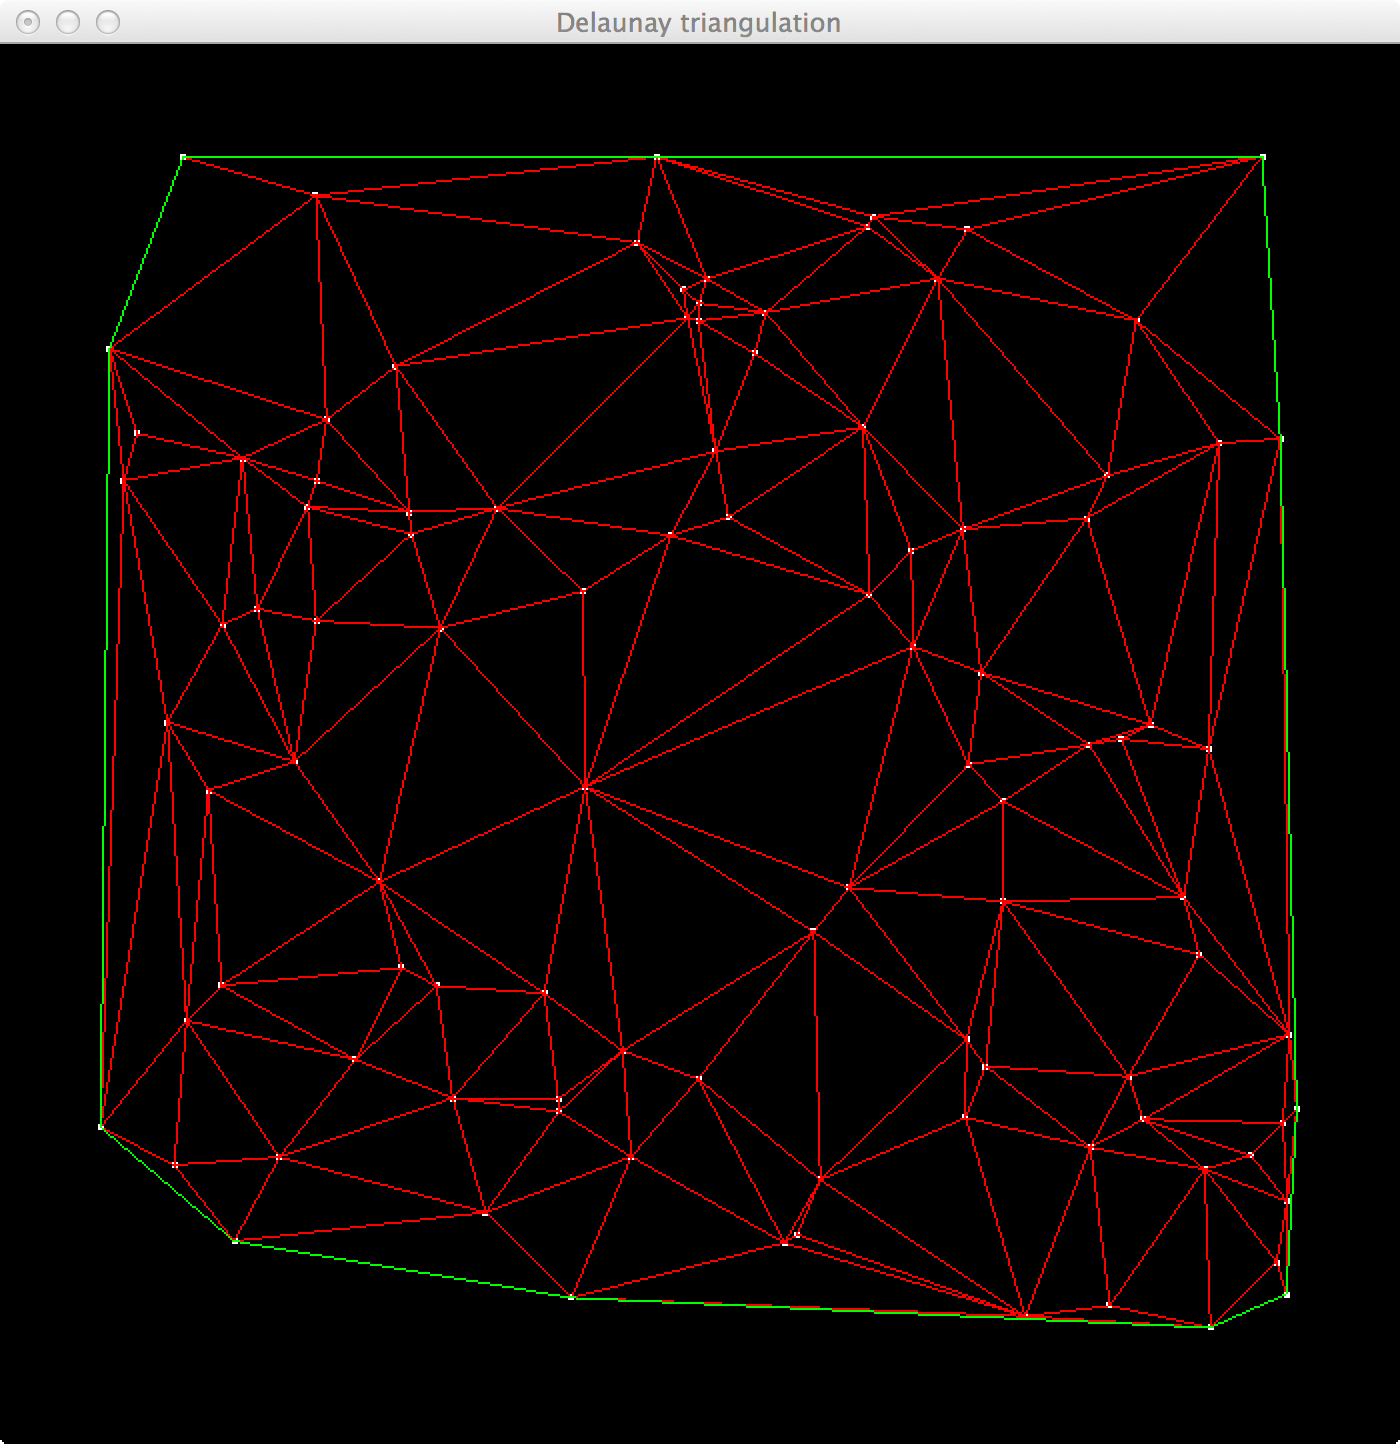
\includegraphics[width=0.9\textwidth]{./img/a_outer_boundary}
		\caption{A Delauny Triangulation with the outer boundary highlighted.}
		\label{fig:a:outer_boundary}		
	\end{minipage}
	\hspace{0.1\textwidth}
	\begin{minipage}[t]{0.45\textwidth}
		\centering
		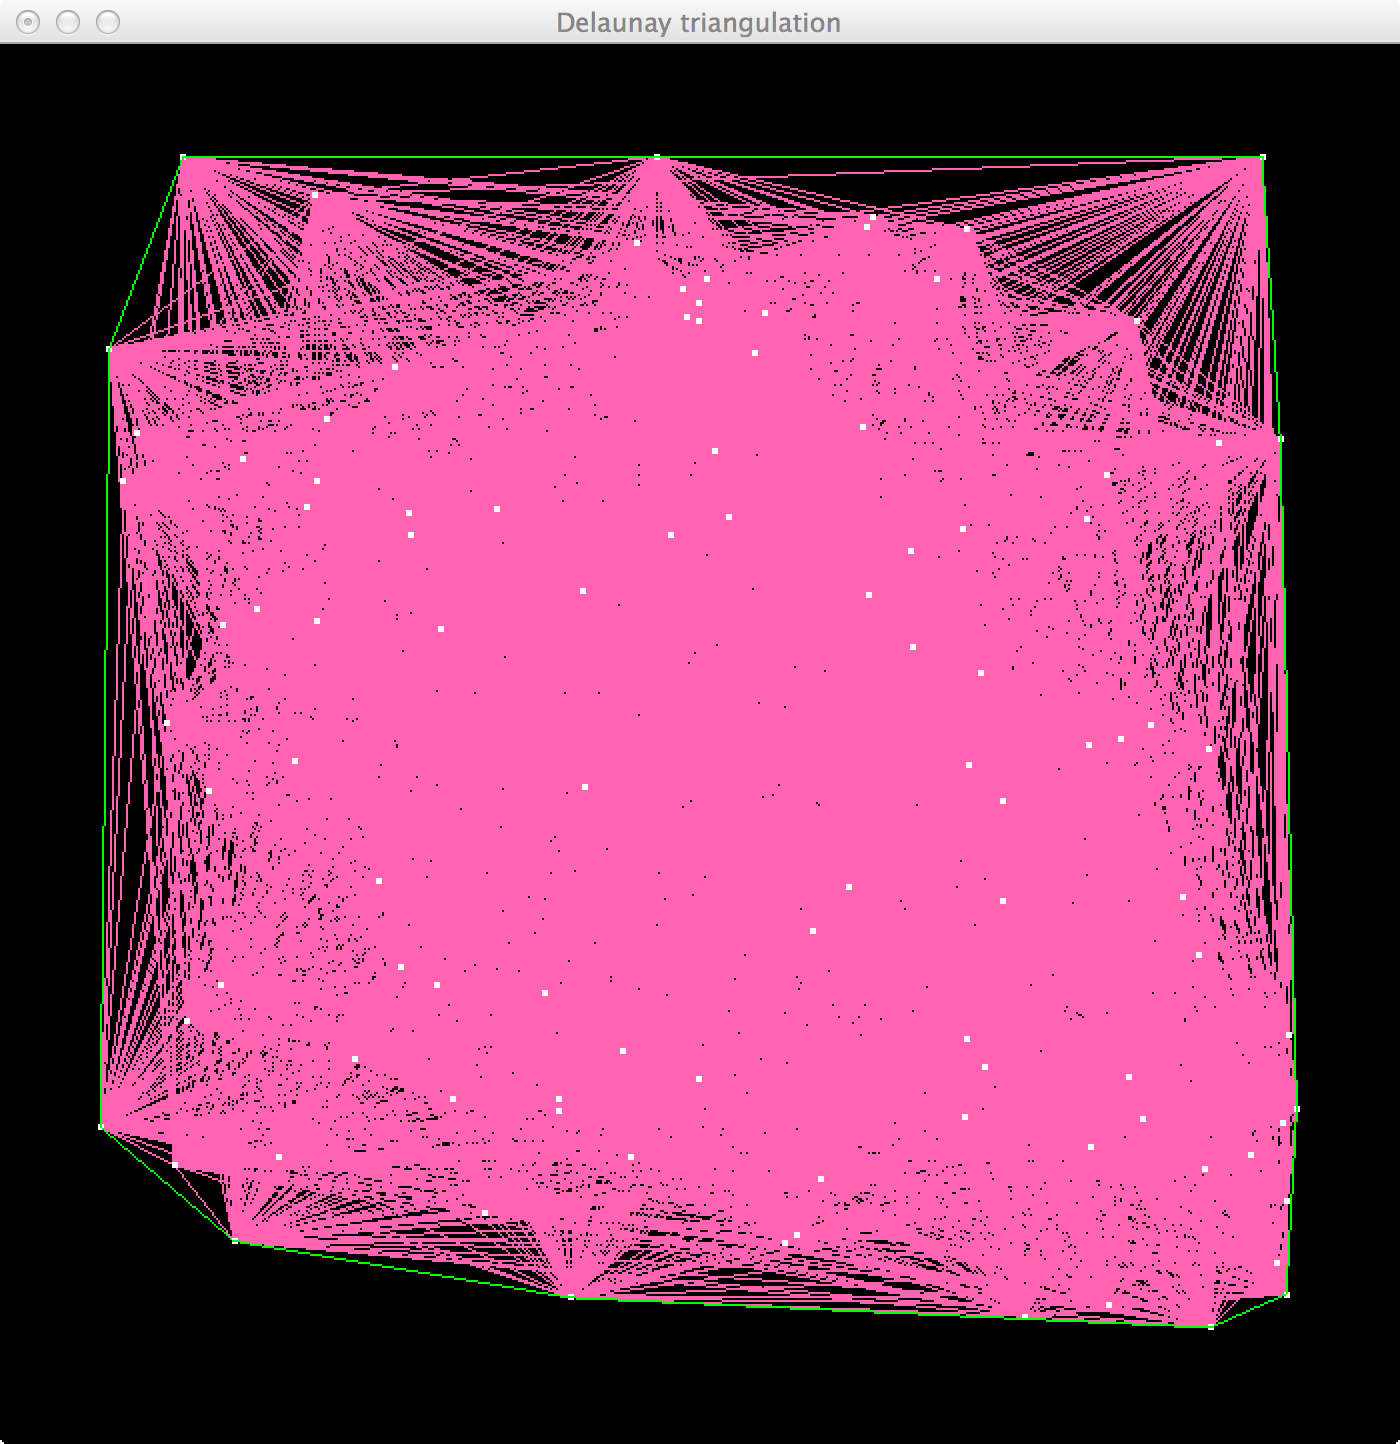
\includegraphics[width=0.9\textwidth]{./img/a_convex_hull}
		\caption{The vertices of the Delauny Triangulation shown in \autoref{fig:a:outer_boundary}, the outer boundary of the triangulation and all possible line segments between the vertices of the triangulation.}
		\label{fig:a:convex_hull}		
	\end{minipage}
\end{figure}
